\documentclass[11pt]{beamer}
\usepackage{tikz}
\usetikzlibrary{positioning}
\usetikzlibrary{shapes, arrows}
\usetheme{metropolis}
\usepackage{graphicx}

% define block styles
\tikzstyle{rounded} = [rectangle, draw, text centered, rounded corners]
\tikzstyle{parallo} = [trapezium,trapezium left angle=70,trapezium right angle=-70, draw, text centered]
\tikzstyle{box} = [rectangle, draw, text centered]
\tikzstyle{line} = [draw, -latex]

\title{Automatic Speech Recognition System}
\subtitle{OOAD Project}
\author{
  Bikash Gupta(070BCT-512)\\
  Kshitiz Shrestha(070BCT-518)\\
  Miran Ghimire(070BCT-521)\\
  Nabin Bhattarai(070BCT-522)\\
  Pabin Raj Luitel(070BCT-523)\\
  Sabin Silwal(070BCT-532)
}
\institute{IOE, Central Campus Pulchowk}
\date{\today}


\begin{document}
\begin{frame}
\titlepage
\end{frame}

\begin{frame}
  \centering
  \frametitle{History Of Speech Recognition}
  \begin{itemize}
  \item 1930s: Bell Lab's investigation in speech perception.
    \pause
  \item 1950s: Single-Speaker digit recognition system.
    \pause
  \item 1960s: Rise of Hidden Markov Model.
    \pause
  \item 1970s: Development of DARPA(Defense Advanced Research Projects Agency) SR.
    \pause
  \item 1980s: Limited vocabulary based speech recognition system.
    \pause
  \item 1990s: First commercially successful speech recognition technologies.
    \pause
  \item $21^{st}$ Century : Effective systems with deep learning and LSTM(Long short-term memory).
  \end{itemize}
\end{frame}

\begin{frame}
  \centering
  \frametitle{Speech Recognition}
  \begin{itemize}
    \pause
  \item Translating spoken words into text.
    \pause
  \item It is very Hard due to
    \pause
    \begin{itemize}
    \item Different Accent, Pronunciations, Styles, Rate of Speaker
      \pause
    \item Noise, different types of microphones.
    \end{itemize}
  \end{itemize}
\end{frame}

\begin{frame}
  \centering
  \frametitle{Usage Of ASR}
  \begin{itemize}
  \item Can be integrated with other digital system to make ease to use
    \pause
  \item Home Automation
    \pause
  \item Hands-free computing
    \pause
  \item Interactive voice response
    \pause
  \item Robotics
    \pause
  \item And Many more...
  \end{itemize}
\end{frame}

\begin{frame}[c]
  \frametitle{Project Overview}
  \centering
  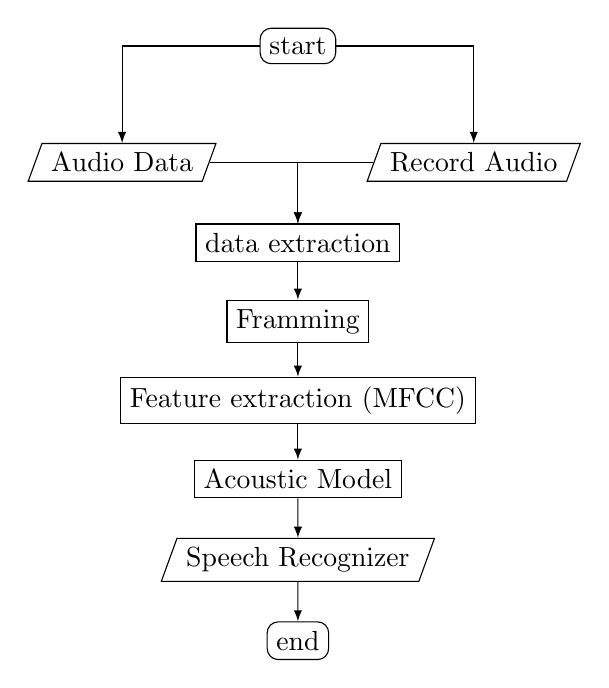
\begin{tikzpicture}[align=center, node distance=1.5cm]
    \node [rounded] (start) {start};
    \node [parallo, below right=1cm and 1.5cm of start] (record_audio)  [ below right=1cm and 1.5cm of start] {Record Audio};
    \node [parallo] (audio_data)  [below left=1cm and 1.5cm of start] {Audio Data};
    \node [box, below of=start, node distance=2.5cm, align=center] (data_ext) {data extraction};
    \node [box, below of=data_ext, node distance=1cm, align=center] (framming) {Framming};
    \node [box, below of=framming, node distance=1cm] (feature_ext) {Feature extraction (MFCC)};
    \node [box, below of=feature_ext, node distance=1cm] (acoustic_model) {Acoustic Model};
    \node [parallo] (speech_recognizer) [below=0.5cm of acoustic_model] {Speech Recognizer};
    \node [rounded] (end) [below=0.5cm of speech_recognizer] {end};

    \path [line] (start) -| (record_audio);
    \path [line] (start) -| (audio_data);
    \path [line] (record_audio) -| (data_ext);
    \path [line] (audio_data) -| (data_ext);
    \path [line] (data_ext) -- (framming);
    \path [line] (framming) -- (feature_ext);
    \path [line] (feature_ext) -- (acoustic_model);
    \path [line] (acoustic_model) -- (speech_recognizer);
    \path [line] (speech_recognizer) -- (end);
  
  \end{tikzpicture}
\end{frame}

\begin{frame}
  \frametitle{Recorder}
  \begin{itemize}
  \item Record audio signal from user and store it in a Audio Object.
  \item We are using python's pyaudio library to record audio signal.
  \item Specifications of Recording
    \begin{itemize}
    \item{Samplerate} : 16000$H_z$
    \item{Channels} : 1 (mono)
    \item{Samplewidth} : 2 Bytes
    \end{itemize}
  \end{itemize}
\end{frame}

% \begin{frame}
%   \frametitle{Audio Object}
%   \begin{itemize}
%   \item It stores audio signal in convenient way for processing.
%   \item Remove Noise from Audio signal.
%   \item Framing the sample data.
%   \item Provides functionalities such as playing audio, information about audio signal
%   \end{itemize}
% \end{frame}

\begin{frame}
  \frametitle{Framing}
  \begin{itemize}
  \item Framing is the process of separating sample data to a series of vector with those sample value
  \item Specifications of frame
    \begin{itemize}
    \item{Frame Duration:}25ms
    \item{Frame Step:}10ms
    \end{itemize}
  \item In our case
    \begin{itemize}
    \item{Frame Size:}400 samples
    \item{Frame Step:}160 samples
    \end{itemize}
  \end{itemize}
\end{frame}

\begin{frame}
  \frametitle{Feature Extraction}
\begin{itemize}
\item Feature extraction is the process of getting data from audio that play main role in speech recognition process.
\item For every frame of sample data, the features are extracted.
\item MFCC Feature extraction
\end{itemize}
  \centering
  \begin{figure}[C]
    \centering
    \includegraphics[width=1\textwidth]{../MFCC_Flowchart.png}
  \end{figure}
\end{frame}
\begin{frame}
  \frametitle{Feed Forward Neural Network}
\end{frame}

\begin{frame}
  \frametitle{Language Model}
  \subtitle{NGram Language Model}
  \begin{itemize}
  \item Used to predict the next word, given previous words.
  \item It gives the probability of next word.
  \item Trained with English books for the model of English language.
  \item Helps to find the spoken words.
  \end{itemize}
\end{frame}
\end{document}
%%% Local Variables:
%%% mode: latex
%%% TeX-master: t
%%% End:
